\documentclass{article}

\usepackage{ctex}
\usepackage[left=1.25in,right=1.25in,top=1in,bottom=1in]{geometry}
\usepackage{amsmath}
\usepackage{amssymb}
\usepackage{graphicx}
\usepackage{float}
\usepackage{subfigure}
\usepackage{listings}
\usepackage{xcolor}
\lstset{language=Python}   
\lstset{breaklines}              
\lstset{extendedchars=false}
\lstset{ 
	backgroundcolor=\color{white},   % 选择代码背景,必须加上\ usepackage {color}或\ usepackage {xcolor}.
	basicstyle=\footnotesize,        % 设置代码字号.
	breakatwhitespace=false,         % 设置是否当且仅当在空白处自动中断.
	breaklines=true,                 % 设置自动断行.
	captionpos=b,                    % 设置标题位置.
	commentstyle=\color{mygreen},    % 设置注释格式
	deletekeywords={...},            % 是否删除给定语言的关键词.
	escapeinside={\%*}{*)},          % 是否在代码中添加LaTex.
	extendedchars=true,              % 是否允许使用非ASCII字符; 仅适用于8位编码,不适用于UTF-8. 
	frame=single,	                   % 给代码区添加边框.
	keepspaces=true,                 % 保留空格(useful for keeping indentation of code (possibly needs columns=flexible).
	keywordstyle=\color{blue},       % 关键字显示风格.
	language=Octave,                 % 使用的语言.
	morekeywords={*,...},            % 是否需要添加其他的关键词.
	numbers=left,                    % 给代码添加行号,可取值none, left, right.
	numbersep=5pt,                   % 设置行号与代码之间的间隔
	numberstyle=\tiny\color{mygray}, % 行号的字号和颜色
	rulecolor=\color{black},         % 边框颜色,如果没有设置,框架颜色可以在非黑色文本中的换行符上更改(例如 text (e.g. comments (green here)))
	showspaces=false,                % 显示每个地方添加特定下划线的空格; 覆盖了'showtringspaces'
	showstringspaces=false,          % 仅在字符串中允许空格
	showtabs=false,                  % show tabs within strings adding particular underscores
	stepnumber=2,                    % the step between two line-numbers. If it's 1, each line will be numbered
	stringstyle=\color{mymauve},     % string literal style
	tabsize=2,	                   % 将默认tab设置为2个空格
	title=\lstname                   % show the filename of files included with \lstinputlisting; also try caption instead of title
}

\usepackage[framed,numbered,autolinebreaks,useliterate]{mcode}

\author{张泽宇}
\date{2022年4月24日}
\title{第八、九周工作总结}

\begin{document}
	\maketitle
	
	
	{\centering \rule[15pt]{15cm}{0.1em}}
	
	{
	\noindent
	\large
	\textbf{过去两周的主要进行的工作包括有:
		\begin{itemize}
			\item 将之前尝试的灰度图像转换程序进行了完善,可由PSCAD输出的.out文件直接转换成灰度图。
			\item 利用灰度图进行网络训练,但是最终的识别效果不好,从不同方面尝试改进。
		\end{itemize}
	}}
	
	以下为详细叙述
	
	{\centering \rule[-10pt]{15cm}{0.1em}}
	
	\newpage
	
	\section{灰度图像转换程序}
	
	程序的主要构造思想如下:
	
	\begin{figure}[h]
		\centering
		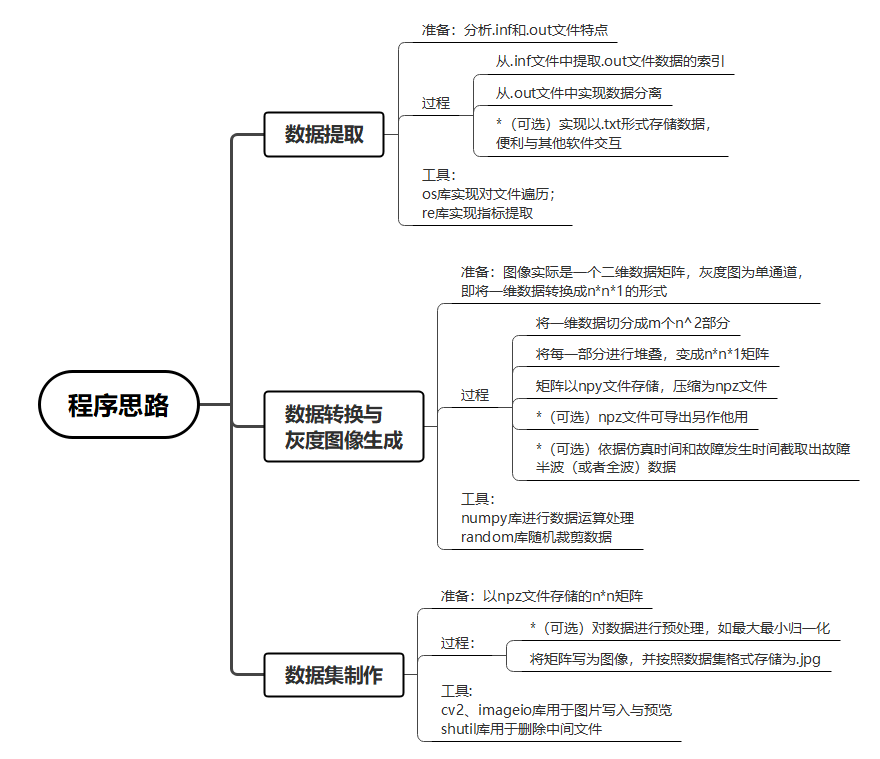
\includegraphics[width=15cm]{figure/程序西路.png}
		\caption{程序思路}
	\end{figure}

	现就每一部分程序进行注解。
	
	\subsection{数据提取}
	
	首先分析一下PSCAD输出数据文件的特点。上几周处理数据时,一直都在关注.infx文件,如下图\ref{fig:infx}所示,其中的数据还是比较繁琐的,有很多不需要关注的信息。后来,通过查阅书籍,发现应该从inf文件中提取相关数据索引。

	\begin{figure}[h]
		\centering
		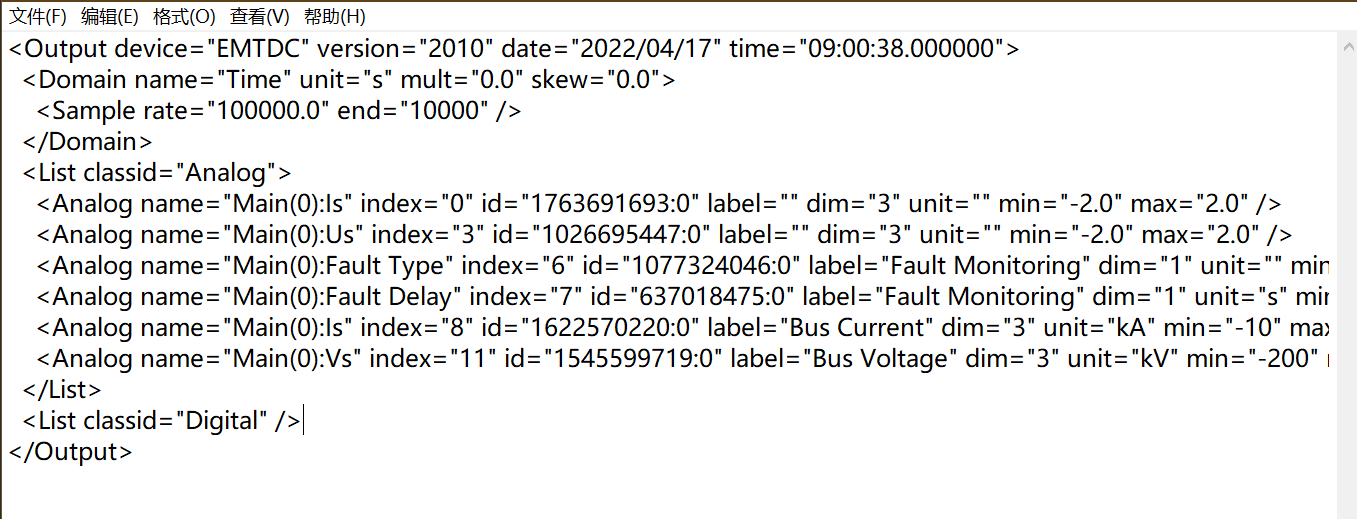
\includegraphics[width=15cm]{figure/infx.png}
		\caption{.infx文件}
		\label{fig:infx}
	\end{figure}

	如图\ref{fig:inf}所示,其中PGB(i)表示.out文件中的第i+1列(第1列是时间);Desc表示该列数据名称,Unit表示单位。因此,利用os库对数据文件进行遍历打开读取操作,采用正则表达式实现对数据名称的提取,并利用列索引将具体数值提取出来,最后以字典的形式暂时存储数据,即可实现对数据的提取。
	
	\begin{figure}[h]
		\centering
		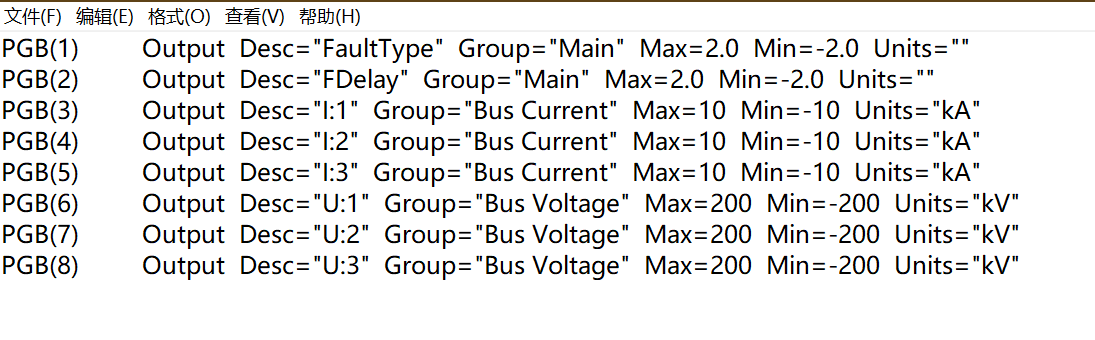
\includegraphics[width=15cm]{figure/inf.png}
		\caption{.inf文件}
		\label{fig:inf}
	\end{figure}

	这部分代码如下所示:
	
	\begin{lstlisting}
	def read_variable_name(f_path):
		L = {}
		f = open(f_path, 'r', encoding='utf-8')
		for line in f:
			reformat = re.compile(r"PGB\((?P<PGB>.*?)\)(.*?)"
			r"(.*?)Desc=\"(?P<Desc>.*?)\"", re.S)
			index = reformat.finditer(line)
			for item in index:
				L[item.group("PGB")] = item.group("Desc").replace(":", "_")
		f.close()
		return L
	
	def read_simulation_time(f_path):
		f = open(f_path, 'r', encoding='utf-8')
		L = []
		for line in f:
			line = line.replace("\n", '')
			line = re.split(r"[ ]+", line)
			if line[1]:
				L.append(line[1])
			else:
				continue
		f.close()
		return L
		
	def read_variable_value(f_path, index):
		f = open(f_path, 'r', encoding='utf-8')
		data_temp = []
		for line in f:
			line = line.replace("\n", '')
			line = re.split(r"[ ]+", line)
			data_temp.append(line)
		f.close()
		column_number = list(index.keys())
		column_name = list(index.values())
		dir_temp = {}
		for i in range(len(column_name)):
			L = []
			for line in data_temp:
				if line[1]:
					L.append(eval(line[eval(column_number[i]) + 1]))
				else:
					continue
			dir_temp[column_name[i]] = L
		return dir_temp
	\end{lstlisting}
	
	程序中有一些步骤是为了处理文件中的细节,如开头空行、间隔不等等问题,待完善注释后上传到Github中。最终返回的dir\_temp是一个字典类型,key是每个项目,如I\_1,value是对应的值。
	
	\subsection{数据转换与图像生成}
	
	首先把一维数据信号截成需要的长度(这里以64$\times$64=4096为例)
	
	\begin{lstlisting}
	def turn_grayscale(data):
		lens = len(data)
		max_start = lens - dimension_grayscale ** 2
		starts = []
		gray_scales = []
		for i in range(sampling_value):
		while True:
			start = random.randint(0, max_start)
			if start not in starts:
				starts.append(start)
				break
			temp = data[start: start + dimension_grayscale ** 2]
			temp = np.array(temp)
			gray_temp = temp.reshape(dimension_grayscale, dimension_grayscale)
			gray_scales.append(gray_temp)
		return gray_scales
	\end{lstlisting}
	
	这里面starts用来存储开始点,共有sampling\_value个开始点,开始点往后dimension\_grayscale ** 2个数据(这里以$64^{2}$为例)提取出来,并转换成ndarray数据形式,再利用reshape函数变成二维矩阵。最终由gray\_scales收集所有的二维矩阵。
	
	其次考虑矩阵数据存贮的问题。这里之所以单独将矩阵数据存储出来,是为了方便其他程序的调用。例如,如果采用PyTorch读取数据,直接读.npz文件要由于读取.img文件。所以加入这段程序,最终数据存在npz.压缩文件中。需要使用时,直接采用load函数即可解压为npy文件并读取成ndarray数据类型。
	\begin{lstlisting}
	def draw_grayscale(graydata, name_npz, up_name, upp_name, uppp_name):
		path_name = r''
		if os.path.exists(path_name):
			np.savez(path_name + '{}'.format(name_npz), *graydata)
		else:
			os.makedirs(path_name)
			np.savez(path_name + '{}'.format(name_npz), *graydata)
		return
	\end{lstlisting}
	
	\subsection{数据集制作}
	
	这部分相对而言较为灵活,利用os库依据需求创建文件夹,并利用imageio向其中写入文件,即可得到所需要的数据集。这里数据集的组成方式,也可以灵活设定,有如下两种方式:
	\begin{itemize}
		\item 分为Train和Test两个文件夹,其下有已分类依据(如故障类型)为名的子文件夹,子文件夹下存储相应的图像文件。
		
		这类方法主要适用于Matlab平台的神经网络。
		
		\item 分为Train\_Image,Test\_Image,Train\_Label,Test\_Label四个文件夹,其中前两个文件夹用于存储照片,后两个以txt文本形式存储标签信息,如故障类型、故障时间、故障地点等。图像文件与文本文件依靠同名的形式相关联。
		
		这种方式更多应用于PyTorch框架。
	\end{itemize}
	
	\begin{lstlisting}
	def divide_dataset(filename, up_name, upp_name, uppp_name):
		npz_file = np.load('',allow_pickle=True)
		for file in npz_file:
			temp = npz_file[file]
			temp = temp.astype(np.float64)
			if up_name == 1:
				path_dir = 'DataSet\\1\\'
			elif up_name == 8:
				path_dir = 'DataSet\\8\\'
			else:
				continue
			img_name = "{0}_{1}_{2}_{3}".format(uppp_name, up_name, upp_name, filename)
			if os.path.exists(path_dir):
				imageio.imwrite(path_dir + img_name + '{}.jpg'.format(file), temp)
			else:
				os.makedirs('' + path_dir)	imageio.imwrite(path_dir + img_name +	'{}.jpg'.format(file), temp)
		return
	\end{lstlisting}
	
	以上即为程序的主要部分(除去一些细枝末节),个人认为这个程序还是具有一定的普适性。当然,程序在一些处理上也存在有可以继续优化提升速率的地方。
	
	
	\section{对灰度图的训练}
	
	灰度图数据的来源依然是上一次搭建的10kV接地小电阻模型。
	
	首先,设置了9个故障点,每个故障点发生A相短路接地、AB相短路接地、三相短路接地、AB相短路四种故障;故障发生时间由起始时间0.01s和延迟时间决定,延迟时间从0开始以0.001为步长变化到0.01.因此总的故障发生时间在0.01~0.02s之间;故障持续时间设置为0.01s,即半个周期。
	
	然后,收集0~0.05s的故障电流与电压数据。利用Multiple Run模块,设置自动运行,最终得到了396次仿真结果,取其中的I\_1即A相电流作为指标生成灰度图。每次运行数据长度为5003个,随机取其中4096个数据生成100个64像素灰度图,用于数据增强。
	
	最后,为简便起见,先判断故障类型。取发生于T1处的数据生成的灰度图作为数据集。如下图所示:
	
	\begin{figure}[h]
		\centering
		\subfigure{
			\begin{minipage}[t]{0.3\linewidth}
				\centering
				
\includegraphics[width=1in]{figure/T1_10000000.0_0.0_I_1arr_0.jpg}
				\caption{A相短路接地}
			\end{minipage}
		}
		\subfigure{
			\begin{minipage}[t]{0.3\linewidth}
				\centering
				
\includegraphics[width=1in]{figure/T1_40000000.0_0.0_I_1arr_0.jpg}
				\caption{AB相短路接地}
			\end{minipage}
		}
		
		\subfigure{
			\begin{minipage}[t]{0.3\linewidth}
				\centering
				
\includegraphics[width=1in]{figure/T1_70000000.0_0.0_I_1arr_0.jpg}
				\caption{ABC三相短路接地}
			\end{minipage}
		}
		\subfigure{
			\begin{minipage}[t]{0.3\linewidth}
				\centering
				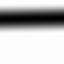
\includegraphics[width=1in]{figure/T1_80000000.0_0.0_I_1arr_0.jpg}
				\caption{AB相短路}
			\end{minipage}
		}
	
	\end{figure}

	发现问题,每个图像之间似乎相似度比较高,只是黑色带出现的位置稍有不同。怀着侥幸心理,利用matlab搭建了网络,结构如下图:
	
	\begin{figure}[h]
		\centering
		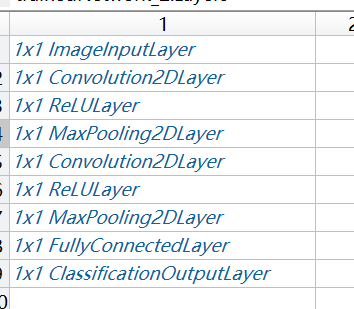
\includegraphics[width=7cm]{figure/nn.png}
		\caption{神经网络}
	\end{figure}

	进行训练,最初出现了损失值为NAN的问题。显示是损失值达到NAN,寻来你只进行了两轮迭代就停止。通过网上论坛,可能的原因一个是学习率太大,我把学习率由0.01降低为0.005,但依旧无法解决;另一个原因可能是梯度爆炸的问题发生。解决梯度爆炸,由于这个结构中已经采用了ReLU激活函数,在不改变网络结构的前提下,只能进行梯度裁剪。所以我设定了一个梯度阈值,最终不再报错。但是尽管如此,说明网络的设计还是有一些问题。
	
	训练结果也说明了这个问题。最后的损失值不收敛,训练集准确率基本不变化,在20\%到30\%之间浮动,验证集的准确率是25\%。
	
	显然,25\%恰为$\frac{1}{4}$,模型识别不了故障类型。
	
	出现这样的表现,我认为可能的问题出在两点,也有可能两方面都有:
	
	\begin{itemize}
		\item 数据集的问题。
		
		事实上,单纯人工去看数据集,发现每个图片的区别实在不能算作显著。
		下面两幅图是A相单相接地和AB相短路的图:
		
		\begin{figure}[h]
			\centering
			\subfigure{
				\begin{minipage}[t]{1\linewidth}
					\centering
					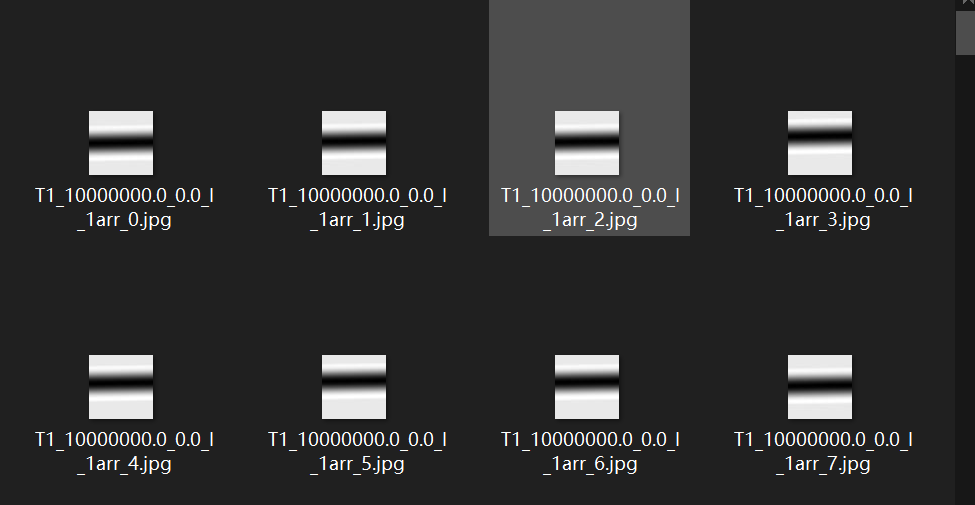
\includegraphics[width=11cm]{figure/11.png}
					\caption{A相短路接地}
				\end{minipage}
			}
			\subfigure{
				\begin{minipage}[t]{1\linewidth}
					\centering
					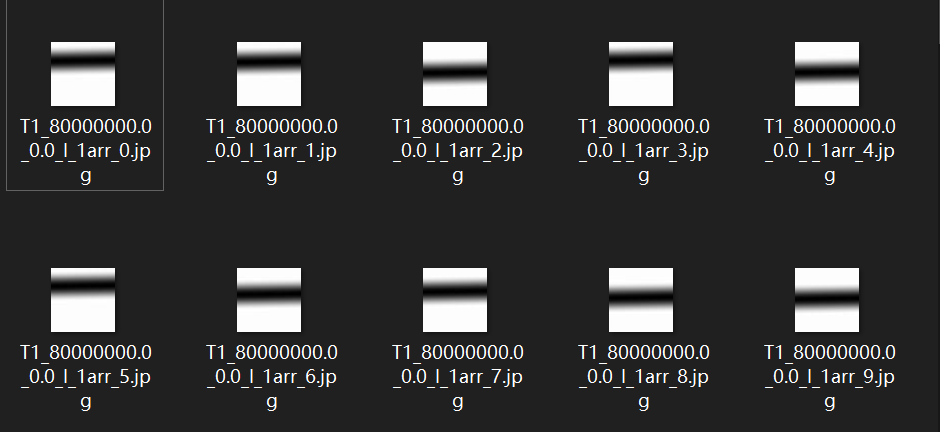
\includegraphics[width=11cm]{figure/88.png}
					\caption{AB相短路接地}
				\end{minipage}
			}
		\end{figure}
	
		发现图像之间太过于相像,自然训练不出什么结果。输出B,C相电流的灰度图,也是基本如此;而ABC三相的电压灰度图,只有三相短路接地的情况下图像有两条黑纹,其他也是类似。我返回去重新看了一下数据结果,发现出现故障的地方,无论是电压还是电流量,大小与正常情况下有大概10的二次方倍数量级,我猜测是这里出现的问题。
		
		因为在转换成灰度图的过程中,矩阵中的每个值按照一定的算法映射在0-256之间,正常与故障之间相差太大,就会导致映射之后正常的数据集中在256附件,故障数据集中在0附近,这样造成了图片中黑白分明,都有一道黑纹的现象。
		
		为了验证我的猜想,我用opencv读取灰度图,得到的是ndarray类型数据,然后将灰度矩阵中的每个元素按照最大最小归一化处理再乘256,两个矩阵进行比较,发现每个元素数值相近。这就说明在生成灰度图的过程中,imageio库采用了最大最小算法或者类似的算法,对每一个数据进行处理,这样的处理是等比例间距的,即使在0-256的空间上,依然保留了每个元素在原始空间上的相对位置。所以,要想解决,一方面可以通过模型的修改,使这个数据之间的数量级差别降低,另一方面可以通过算法的修改,(比方采用标准差方式映射到0-256之间?只是一个猜想)。这两个方向下一周计划进行尝试。
		
		\item 另一个方面,在神经网络上。
		
		梯度爆炸的产生是因为反向传播的过程中梯度不断累计,以指数级增长,导致网络无法训练。采用ReLU激活函数是解决的一个办法,但是在本例中显然ReLU没有发挥应有的作用。但是反过来看网络的结构,参数设置并没有很复杂,网络深度也不大,那出现梯度爆炸的原因,会不会是由于数据的问题?这一点还待探讨。
	
		关于灰度图的问题,我在网上也找了一些资料,其中有一个“基于卷积神经网络的数据驱动故障预测方法”\footnote{https://www.sci-hub.ren/10.1109/tie.2017.2774777},这个方法也是采用灰度图进行故障检测,我利用它的数据生成了灰度图如下:
			
		\begin{figure}[h]
			\centering
			\subfigure{
				\begin{minipage}[h]{0.48\linewidth}
					\centering
					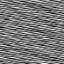
\includegraphics[width=5cm]{figure/arr_0.jpg}
					\caption{A类}
				\end{minipage}
			}
			\subfigure{
				\begin{minipage}[h]{0.48\linewidth}
					\centering
					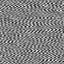
\includegraphics[width=5cm]{figure/arr_1.jpg}
					\caption{B类}
				\end{minipage}
			}
		\end{figure}
	
		能看得出来,这两类的灰度图之间差别还是比较明显的。因此我认为主要的问题还是出现在对数据的处理上,可能神经网络是没有问题,而是由于数据太过于特殊导致无法正常训练。
	\end{itemize}
	
	总而言之,下一周将会对数据集的处理进行进一步探讨。

\end{document}